\documentclass{article}
\usepackage[utf8]{inputenc}
\usepackage{polski}
\usepackage{graphicx}
\usepackage{hyperref}


\begin{document}

\begin{titlepage}
\newcommand{\HRule}{\rule{\linewidth}{0.5mm}}
\begin{center}
\textsc{\LARGE Politechnika Warszawska}\\[0.5cm]
\textsc{\Large Wydział Matematyki i Nauk Informacyjnych}\\[1cm]

\includegraphics[width=2cm, height=2cm]{logo}\\[1cm]
\textsc{\Huge Sieci neuronowe}\\[0.5cm]
\HRule \\[0.4cm]
{ \LARGE \bfseries Rozpoznawanie i klasyfikacja pisanych cyfr przy użyciu modeli matematycznych - raport}\\[4cm]
\begin{flushright}
\Large \emph{Autorzy:}\\[0.5cm]
Anna \textsc{Zawadzka}\\
Piotr \textsc{Waszkiewicz}\\[2.5cm]
\end{flushright} 
\vfill
{\large \today}\\[1cm]	
\end{center}
\end{titlepage}

\newpage
%----------------------------------------------------------------------------------------
\section{Opis problemu badawczego}
Problem badawczy przedstawiony na stronie \textit{https://www.kaggle.com/c/digit-recognizer} polega na rozpoznawaniu i klasyfikacji ręcznie pisanych cyfr poprzez przetwarzanie i analizę obrazów przedstawiających odpowiednie symbole. Zbiory danych zostały zaczerpnięte z publicznej bazy danych  MNIST\cite{mnist_database}. 
\begin{center}
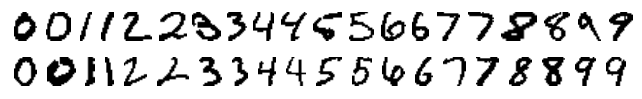
\includegraphics[width=0.49\textwidth]{native}
\end{center}

\section{Cel badań}
Projekt zakładał realizację zadania poprzez zbadanie różnych metod, ze szczególnym uwzględnieniem różnych modeli sieci neuronowych. Zbadane zostały dwa rodzaje takich sieci - Backpropagation oraz SoftMax. Wykorzystane zostały również jedne z najpopularniejszych obecnie klasyfikatorów: maszyny wektorów podpierających (SVM)\cite{CortesVapnik1995}, Lasy Losowe\cite{RF}, kNN\cite{Altman1992}.

Celem badań było porównanie jakości klasyfikacji dla różnych modeli klasyfikatorów i wskazanie najskuteczniejszego pod względem czasu uczenia, wydajności i jakości udzielanych odpowiedzi. Oprócz tego badania miały na celu rozszerzenie istniejącego wektora cech o nowe, unikalne wartości które, jak przypuszczano, polepszyłyby jakość klasyfikacji. W trakcie obliczeń podjęta została próba odrzucenia tych cech które przeszkadzają lub pogarszają działanie modeli. \\


\section{Opis danych}

Zbiory danych treningowych oraz testowych pochodzą z publicznej bazy danych MNIST\cite{mnist_database}. Każdy element ze zbioru treningowego jest opisany 785 wartościami. Pierwsza liczba określa zakodowaną cyfrę (wartość z przedziału [0, 9]), kolejne 784 wartości są z przedziału [0, 255] i opisują kolory pikseli zeskanowanej cyfry w skali szarości dla obrazka o wymiarach 28x28 pikseli. Zbiór testowy w przeciwieństwie do treningowego nie zawiera informacji o reprezentowanej klasie. Zbiór treningowy i testowy zawierają odpowiednio 42,000 i 28,000 elementów. \\

\section{Operacje graficzne}
\label{features_vector}
Jednym z założeń dotyczącym zbioru danych było podjęcie próby zmiany wektora cech poprzez dodanie do niego nowych wartości. Zaproponowane zostały cztery nowe cechy którymi były: liczba punktów startowych cyfry, liczba punktów przecięcia cyfry, wektor przecięć cyfry (opisany dokładniej w podrozdziale \ref{DigitIntersectionVector}) a także informacja o liczbie czarnych pikseli. Wszystkie wymienione wyżej cechy zostały wyliczone na podstawie szkieletu litery znajdującej się na obrazku, będącego wynikiem operacji zwanej szkieletyzacją. 

\subsection{Dylatacja}
Dylatacja to operacja morfologiczna która służy do zamykania małych otworów oraz zatok we wnętrzu symbolu. Obiekty zwiększają swoją objętość i jeśli dwa lub więcej obiektów położonych jest blisko siebie, zrastają się w jedną, większą całość.

\subsection{Erozja}
Erozja jest operacją odwrotną do dylatacji. Jej działanie polega na obcinaniu brzegów obiektu na obrazie.

\subsection{Szkieletyzacja}
Szkieletyzacja, zwana również operacją ścieniania, służy do odchudzania graficznego symbolu tak aby jako wynik otrzymać ten sam symbol narysowany linią o grubości jednego piksela. Obecnie istnieje wiele różnych algorytmów szkieletyzacji różniących się podejściem do zagadnienia, stosowalnością (bywają symbole lepiej ścieniane przez jeden algorytm podczas gdy inne mogą być przez niego odchudzane niepoprawnie) jak i złożonością. Do najbardziej znanych zaliczyć można algorytm \href{http://matwbn.icm.edu.pl/ksiazki/amc/amc20/amc2029.pdf}{K3M}, algorytm \href{https://rosettacode.org/wiki/Zhang-Suen_thinning_algorithm}{Zhang-Suen'a}, algorytm Guo-Hall’a a także algorytm KMM.

\subsection{Znajdowanie punktów startowych cyfry \protect\footnote{Na podstawie artykułu: \href{https://arxiv.org/pdf/1202.3884.pdf}{https://arxiv.org/pdf/1202.3884.pdf} } }
Zazwyczaj pisząc symbole rozpoczynamy i kończymy tę czynność w pewnych szczególnych miejscach. Są to najczęściej niepołączone zakończenia linii które zmuszają do oderwania pióra. Punkty te nazywane są punktami startowymi (chociaż równie dobrze mogłyby nazywać się punktami końcowymi) a ich liczba pomaga w identyfikacji narysowanego symbolu.

\subsection{Znajdowanie przecięć w cyfrze \protect\footnote{Na podstawie artykułu: \href{https://arxiv.org/pdf/1202.3884.pdf}{https://arxiv.org/pdf/1202.3884.pdf} } }
Punktami przecięcia w narysowanym symbolu nazywane są te miejsca w których następuje rozwidlenie ścieżek. Przykładem może być daszek litery T która swój punkt przecięcia posiada w miejscu złączenia daszka i nogi litery. Stosując algorytm opisany w artykule zaimplementowana została funkcjonalność liczenia punktów przecięć w cyfrach.

\subsection{Wektor przecięć cyfry}
\label{DigitIntersectionVector}
Wektor przecięć cyfry zawiera sześć elementów. Przechowuje on wartości informujące o liczbie przecięć narysowanej cyfry z liniami prostymi przechodzącymi przez obraz w określonych miejscach, to znaczy w 30\% 50\% i 70\% jego szerokości i wysokości.

\section{Opis wykorzystanych klasyfikatorów}

\subsection{Backpropagation}
Algorytm wstecznej propagacji błędu jest algorytmem uczenia dla wielowarstwowych sieci neuronowych. Architektura sieci jest zadana z góry, przed przystąpieniem procesu uczenia ustalona jest liczba warstw ukrytych, neuronów w każdej warstwie, neuronów wejściowych i wyjściowych. Główną zaletą algorytmu jest brak konieczności ustalania wag połączeń między neuronami, które są dobierane za pomocą metody obliczeniowej zwanej wsteczną propagacją błędu. Jest to metoda umożliwiająca modyfikację wag w sieci o architekturze warstwowej, we wszystkich jej warstwach.\\\\
Ogólny schemat procesu trenowania sieci wygląda następująco:
\begin{enumerate}
\item Ustalenie topologii sieci
\item Zainicjowanie wag w sposób losowy
\item Obliczenie odpowiedzi sieci dla danego wektora uczącego (warstwa po warstwie)
\item Każdy neuron wyjściowy oblicza swój błąd, oparty na różnicy pomiędzy obliczoną odpowiedzią oraz poprawną odpowiedzią
\item Błędy propagowane są do wcześniejszych warstw
\item Każdy neuron (również w warstwach ukrytych) modyfikuje wagi na podstawie wartości błędu i wielkości przetwarzanych w tym kroku sygnałów
\item Następuje powtórzenie kroków począwszy od punktu 3. dla kolejnych wektorów uczących. Gdy wszystkie wektory zostaną użyte, losowo zmienia się ich kolejność i wykorzystuje się je powtórnie
\item Algorytm zatrzymuje się, gdy średni błąd na danych treningowych osiągnie zadaną wartość (zmaleje wystarczająco)
\end{enumerate}

\subsection{SoftMax}
Softmax jest uogólnieniem regresji logistycznej do przypadku, gdy rozważa się wiele klas. W regresji logistycznej zakłada się, że etykiety są binarne : $y(i) \in \{0,1\}$. Metoda Softmax pozwala obsługiwać $y(i) \in \{1, ..., K\}$ gdzie K jest liczbą klas.
\subsection{SVM}
Metoda maszyny wektorów podpierających (Support Vector Machines) jest jedną z metod uczenia nadzorowanego. Klasyfikator ten znajduje hiperpłaszczyznę rozdzielającą dane treningowe na dwie klasy w ten sposób, że maksymalizuje wartość marginesu geometrycznego dla wszystkich punktów treningowych. Marginesem geometrycznym hiperpłaszczyzny H jest jej odległość do najbliższych punktów. Punkty położone najbliżej hiperpłaszczyzny nazywane są wektorami wspierającymi (ang. support vectors).
\begin{figure}[htp]
	\centering
	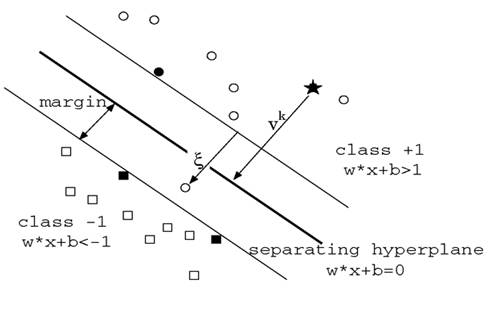
\includegraphics[width=1\textwidth]{Figures/svm.jpg}
	\caption{Schemat działania maszyny wektorów podpierających }
\end{figure}
\subsection{Lasy losowe}
Metoda lasów losowych opiera się na drzewach decyzyjnych, zwanych również drzewami klasyfikacyjnymi. Opierają się one o drzewiastą strukturę, w której węzły wewnętrzne zawierają testy na wartościach atrybutów. Z każdego węzła wewnętrznego wychodzi tyle gałęzi, ile jest możliwych wyników testu w tym węźle.  Klasyfikacja zaczyna się w korzeniu drzewa, a kończy po osiągnięciu jednej z klas terminalnych, czyli liścia.\\ 
Lasy losowe (ang. random forests) będące  uogólnieniem idei drzew decyzyjnych zalicza się do procedur agregujących (ang. ensemble method), w których rolę modelu klasyfikacyjnego pełni grupa modeli składowych. Działanie lasów losowych polega na klasyfikacji za pomocą grupy drzew decyzyjnych. Końcowa decyzja jest podejmowana w wyniku  głosowania większościowego  nad klasami wskazanymi przez poszczególne drzewa decyzyjne.
\begin{figure}[htp]
	\centering
	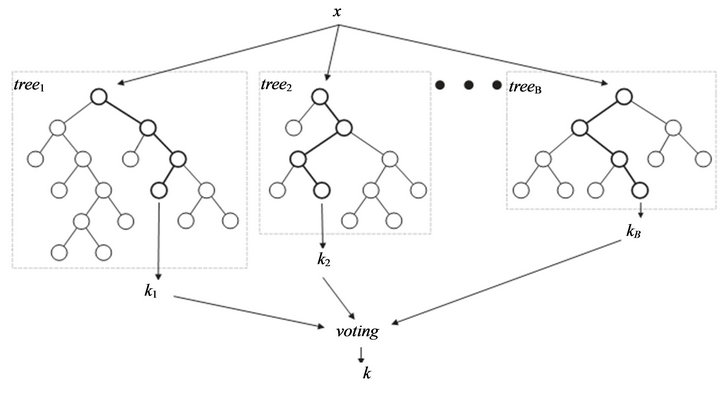
\includegraphics[width=1\textwidth]{Figures/rf.jpg}
	\caption{Schemat działania lasów losowych }
\end{figure}

\subsection{kNN}
Algorytm k najbliższych sąsiadów (ang. k Nearest Neighbours) należy do grupy algorytmów opartych o analizę przypadku. Algorytmy te prezentują swoją wiedzę o świecie w postaci zbioru przypadków lub doświadczeń. Idea klasyfikacji polega na metodach wyszukiwania tych zgromadzonych przypadków, które mogą być zastosowane do klasyfikacji nowych sytuacji. Klasyfikacja nowych przypadków zgodnie z algorytmem kNN jest realizowana na bieżąco, tzn. wtedy gdy pojawia się potrzeba klasyfikacji nowego przypadku, metoda ta nie buduje klasyfikatora. \\
Obiekty są analizowane w ten sposób , że oblicza się odległości bądź podobieństwa między nimi. Istnieją różne miary podobieństwa czy odległości. Powinny być one wybierane konkretnie dla typu danych analizowanych, ponieważ inne są miary typowo dla danych binarnych, inne dla danych nominalnych a inne dla danych numerycznych.\\
Dany jest zbiór uczący zawierający obserwacje z których każda ma przypisany wektor zmiennych objaśniających oraz wartość zmiennej objaśnianej Y oraz dana jest obserwacja C z przypisanym wektorem zmiennych objaśniających dla której chcemy prognozować wartość zmiennej objaśnianej Y.\\
Dla tak zdefiniowanego zadania przebieg algorytmu wygląda następująco:
\begin{enumerate}
\item Porównanie wartości zmiennych objaśniających dla obserwacji C z wartościami tych zmiennych dla każdej obserwacji w zbiorze uczącym
\item Wybór k (ustalona z góry liczba) najbliższych do C obserwacji ze zbioru uczącego
\item Uśrednienie wartości zmiennej objaśnianej dla wybranych obserwacji, w wyniku czego uzyskiwana jest prognoza
\begin{figure}[htp]
	\centering
	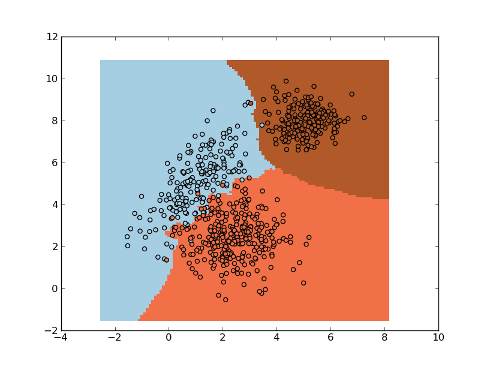
\includegraphics[width=1\textwidth]{Figures/knn.png}
	\caption{Schemat działania metody k najbliższych sąsiadów }
\end{figure}
\end{enumerate}

\section{Opis wyników}
Wyniki zaprezentowane w tym rozdziale zostały uzyskane dla dwóch sposobów otrzymywania wektorów cech. Pierwszy z nich zakładał wykorzystanie obrazów dostępnych w ramach zbiorów testowych i traktowanie ich jako jedynego wejścia dla klasyfikatorów. Drugi sposób rozszerzał wektor o zbiór wyekstrahowanych cech, które zostały opisane w rozdziale \ref{features_vector}. Dla obu podejść dokonano pełnych testów dla każdego z przygotowanych klasyfikatorów. Poniżej zamieszczone zostały tabelki zawierające wyniki. Każda kolumna oznaczona cyfrą oznacza wyniki dla obiektów z danych testowych reprezentujących tę cyfrę. Wartości w komórkach oznaczają jakość klasyfikacji dla poszczególnych klasyfikatorów (ich skuteczność). Wartości w kolumnie oznaczonej jako \textit{error} przestawiają ogólny procent błędu dla każdego z klasyfikatorów. Wiersz \textit{summary} zawiera wartości oznaczające skuteczność rozpoznawania każdej z cyfr przez klasyfikatory łącznie.

\begin{table}[htp]
	\centering
	\caption{Wyniki dla danych z podstawowym wektorem cech}
	\label{basic-vector-results}
\begin{tabular}{l|l|l|l|l|l|l|l|l|l|l|l|}
	\cline{2-12}
	& \textbf{0} & \textbf{1} & \textbf{2} & \textbf{3} & \textbf{4} & \textbf{5} & \textbf{6} & \textbf{7} & \textbf{8} & \textbf{9} & \textbf{error} \\ \hline
	\multicolumn{1}{|l|}{\textbf{SoftMax}}         & 0.86       & 0.83       & 0.84       & 0.83       & 0.81       & 0.80       & 0.85       & 0.84       & 0.80       & 0.81       & 0.17                \\ \hline
	\multicolumn{1}{|l|}{\textbf{Backpropagation}} & 0.83       & 0.85       & 0.80       & 0.82       & 0.80       & 0.79       & 0.83       & 0.82       & 0.79       & 0.79       & 0.19                \\ \hline
	\multicolumn{1}{|l|}{\textbf{SVM}}             & 0.20       & 0.92       & 0.00       & 0.52       & 0.45       & 0.00       & 0.68       & 0.12       & 0.00       & 0.81       & 0.80                \\ \hline
	\multicolumn{1}{|l|}{\textbf{RF}}              & 0.89       & 0.91       & 0.86       & 0.88       & 0.88       & 0.88       & 0.90       & 0.89       & 0.87       & 0.87       & 0.12                \\ \hline
	\multicolumn{1}{|l|}{\textbf{kNN}}             & 0.88       & 0.86       & 0.89       & 0.88       & 0.89       & 0.86       & 0.89       & 0.87       & 0.90       & 0.87       & 0.12                \\ \hline
	\multicolumn{1}{|l|}{\textbf{summary}}         & 0.73       & 0.87       & 0.68       & 0.79       & 0.77       & 0.67       & 0.83       & 0.71       & 0.67       & 0.83       &                     \\ \hline
\end{tabular}
\end{table}

\begin{table}[htp]
	\centering
	\caption{Wyniki dla danych z rozszerzonym wektorem cech}
	\label{extended-vector-results}
\begin{tabular}{l|l|l|l|l|l|l|l|l|l|l|l|}
	\cline{2-12}
	& \textbf{0} & \textbf{1} & \textbf{2} & \textbf{3} & \textbf{4} & \textbf{5} & \textbf{6} & \textbf{7} & \textbf{8} & \textbf{9} & \textbf{error} \\ \hline
	\multicolumn{1}{|l|}{\textbf{SoftMax}}         & 0.65          & 0.61          & 0.62          & 0.62          & 0.62          & 0.60          & 0.63          & 0.63          & 0.61          & 0.59          & 0.38                \\ \hline
	\multicolumn{1}{|l|}{\textbf{Backpropagation}} & 0.49          & 0.48          & 0.45          & 0.47          & 0.47          & 0.43          & 0.49          & 0.46          & 0.44          & 0.45          & 0.54                \\ \hline
	\multicolumn{1}{|l|}{\textbf{SVM}}             & 0.00          & 0.70          & 0.00          & 0.19          & 0.14          & 0.17          & 0.35          & 0.11          & 0.00          & 0.56          & 0.78                \\ \hline
	\multicolumn{1}{|l|}{\textbf{RF}}              & 0.67          & 0.67          & 0.64          & 0.65          & 0.66          & 0.65          & 0.67          & 0.66          & 0.64          & 0.63          & 0.35                \\ \hline
	\multicolumn{1}{|l|}{\textbf{kNN}}             & 0.58          & 0.58          & 0.60          & 0.62          & 0.63          & 0.63          & 0.64          & 0.63          & 0.65          & 0.61          & 0.38                \\ \hline
	\multicolumn{1}{|l|}{\textbf{summary}}         & 0.48          & 0.61          & 0.46          & 0.51          & 0.50          & 0.49          & 0.56          & 0.50          & 0.47          & 0.57          &                     \\ \hline
\end{tabular}
\end{table}

\begin{figure}[htp]
	\centering
	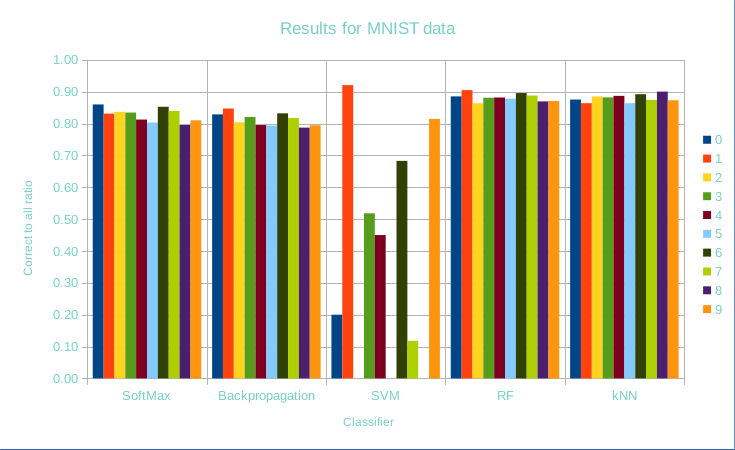
\includegraphics[width=1\textwidth]{Figures/basic-vector-summary.png}
	\caption{ Wyniki dla danych z podstawowym wektorem cech przedstawione na wykresie }
	\label{fig:basic-vector-summary}\vspace{-3pt}
\end{figure}

\begin{figure}[htp]
\centering
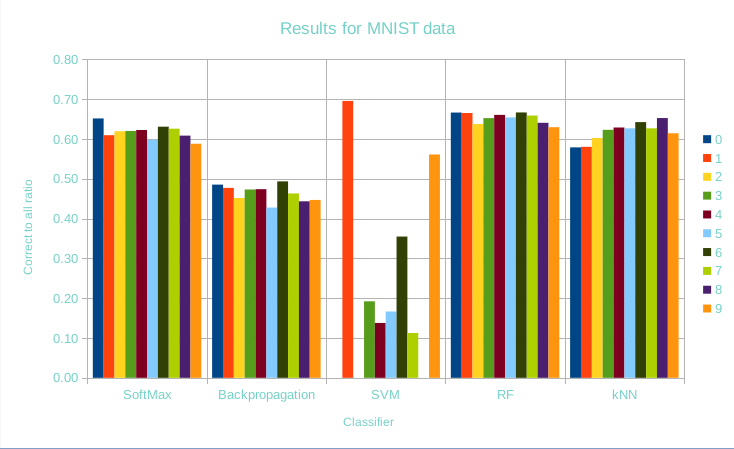
\includegraphics[width=1\textwidth]{Figures/extended-vector-summary.png}
\caption{ Wyniki dla danych z rozszerzonym wektorem cech przedstawione na wykresie }
\label{fig:extended-vector-summary}\vspace{-3pt}
\end{figure}

\section{Podsumowanie}
Wbrew oczekiwaniom rozszerzenie wektora cech wcale nie poprawiło jakości klasyfikacji. Wręcz przeciwnie, wyniki otrzymane dla dodatkowych danych są o wiele gorsze niż te dla samego obrazu. Podczas inspekcji zauważono, że skany cyfr dostarczane jako dane testowe nie poddają się łatwej obróbce graficznej. Próby ustalenia wspólnej maski dla operacji dylatacji i erozji nie przyniosły oczekiwanych rezultatów. Niezależnie od przyjętych wartości zawsze wykonanie którejś z czynności morfologicznej powodowało utratę danych na pewnych obrazach. To z kolei przyczyniło się do uzyskania miernych wyników.

\newpage
\begin{thebibliography}{9}
	\bibitem{mnist_database} LeCun, Y., Cortes, C., and Burges, C., \emph{The MNIST database of handwritten digits}, in: http://yann.lecun.com/exdb/mnist.
	\bibitem{RF} Breiman, L., \emph{Random Forests}. Machine Learning 45 (1), 2001
	\bibitem{CortesVapnik1995} Cortes, C., Vapnik, V., \emph{Support-vector networks}. Machine Learning 20 (3), 1995.	
	\bibitem{Altman1992} Altman N. S., \emph{An introduction to kernel and nearest-neighbor nonparametric regression}. The American Statistician 46 (3), 1992.
    \bibitem{ScholkopfWilliamsonSmola1992} Scholkopf, B., Williamson, R., Smola, A., Shawe-Taylort, J., Platt, J., \emph{Support Vector Method for Novelty Detection}, Advances in Neural Information Processing Systems 12, 1992. 
    \bibitem{WangCasasent2009} Wang, Y., Casasent, D., \emph{A Support Vector Hierarchical Method for multi-class classification and rejection}, Proc. of Int. Joint Conf. on Neural Networks, 2009.
    \bibitem{digit-starting-intersection-points} Dinesh Dileep \emph{A feature extraction technique based on character geometry for character recognition}, \href{https://arxiv.org/pdf/1202.3884.pdf}{https://arxiv.org/pdf/1202.3884.pdf}
    \bibitem{gridsearch} \href{http://scikit-learn.org/stable/modules/grid\_search.html}{http://scikit-learn.org/stable/modules/grid\_search.html}


\end{thebibliography}

\end{document}